% ============================================================
\chapter{A3 and Evaluation: Decomposing the Gain}
\label{chap:evaluation}
% ============================================================

This chapter evaluates (A3, addressing C3). It proceeds Socratically through
the questions Q decomposes into: how should the gain be measured at all
(Section~\ref{sec:method}); does the causal graph improve on the correlation
matrix in the first place --- requirement R1 --- and what happened to the
driver route this project began from (Section~\ref{sec:r1}); how does the
gain split between skeleton and orientation --- the answer to Q ---
and how robust is that split (Section~\ref{sec:decomposition}); and how much
of all of it survives rigorous, multiplicity-aware inference
(Section~\ref{sec:believe-rigour}). Section~\ref{sec:believe} closes with the
threats to validity.

\section{How should the gain be measured?}
\label{sec:method}

\paragraph{Protocol.} Every configuration runs the identical walk-forward
backtest: the fixed 99-name universe, monthly rebalancing over 2007--2024
(215 rebalances), estimation windows of 252 and 504 trading days for both the
graph fit and the sample covariance, weights held for 21 trading days,
transaction costs of 5\,bps per unit of one-way turnover (swept over
$\{0,5,10,20\}$\,bps). ``Performance'' always means the \emph{out-of-sample,
net-of-cost, annualised Sharpe ratio of daily portfolio returns}, reported
alongside CAGR, maximum drawdown and mean turnover; no in-sample or gross
number appears anywhere in this report.

\paragraph{Inference.} Pairwise contrasts use the Politis--Romano stationary
block bootstrap \cite{politis1994stationary} (2000 resamples, mean block 21
days), which resamples the joint return panel so cross-strategy correlation
is preserved. Because daily returns here are heavily non-normal (excess
kurtosis ${\approx}\,\rsKurtosis$; Figure~\ref{fig:retdist}) and because this
project evaluated \rsNtrials\ distinct configurations in total, pairwise
$p$-values are never taken at face value: every claim is re-adjudicated by
the battery of Section~\ref{sec:believe-rigour} --- Probabilistic and
Deflated Sharpe ratios \cite{bailey2012psr,bailey2014deflated} (the DSR
deflating against \emph{all} \rsNtrials\ trials), White's Reality Check
\cite{white2000reality}, Hansen's SPA \cite{hansen2005spa} for each
family-wise comparison, and the $90\%$ Model Confidence Set
\cite{hansen2011mcs}. Regimes are defined by NBER recession dates and
top/bottom VIX quintiles.

\paragraph{Stability.} Two further checks target the failure modes of the
incumbent framework specifically. The \emph{seed audit} re-runs the complete
driver-route pipeline under \rsSeedN\ different neural-network seeds with
everything else frozen, measuring how much of its performance is
initialisation noise (Section~\ref{sec:seed-audit}); the D-family needs no
such audit, being deterministic --- consecutive runs are byte-identical, a
property verified by the replication gate
(Section~\ref{sec:ablation-design}). And every number in this chapter comes
from the bit-reproducible pipeline of Section~\ref{sec:cache}.

\begin{figure}[tbp]
  \centering
  
\includegraphics[width=0.7\textwidth]{figures/returns_distribution.png}
  \caption{Distribution of daily net returns (pooled across variants) against
    a fitted normal, log-density axis. The heavy tails (excess kurtosis
    ${\approx}\,\rsKurtosis$) are why the plain Sharpe ratio is supplemented
    by the Probabilistic and Deflated Sharpe ratios throughout.}
  \label{fig:retdist}
\end{figure}

\section{R1: does the causal graph improve on the correlation matrix at
all?}
\label{sec:r1}

Requirement R1 asks whether there is any gain to decompose. The like-for-like
comparison is the graph-blind \textsc{corr} control against the
skeleton-only D0 on the same allocator: at the one-year window
$\textsc{corr}=\rsCorrSharpe$ against $\text{D0}=0.403$, a skeleton gain of
$+0.022$ ($p=0.14$); adding orientation lifts the best cell to D1's $0.411$,
a total causal-graph gain of $+0.031$ ($p=0.14$). At the two-year window
$\textsc{corr}=\rsCorrSharpeWfive$ and the total gain is $+0.032$--$0.036$
(D1/D2s, $p=0.12$/$0.08$). Every one of the twelve D-versus-\textsc{corr}
contrasts is positive --- consistent in direction across allocators, methods
and windows --- but \emph{none is individually significant}, and the
family-wise test (Hansen's SPA, all causal-structure strategies against
\textsc{corr}) gives $p=\rsSpaSkelWtwo$ at one year and $p=\rsSpaSkelWfive$
at two. R1 is therefore supported directionally but not statistically: the
causal graph consistently out-performs the correlation matrix by a modest
margin that data-snooping correction cannot distinguish from a lucky search.

Two contextual facts sharpen this reading. First, an earlier phase of this
project reported the same comparison against the HSP baseline V0
(correlation-\emph{selected} drivers plus neural sensitivities) and found it
strongly significant ($+0.032$, $p<0.001$; family-wise
$p=\rsSpaConsistent$). The \textsc{corr} control explains the discrepancy:
plain correlation-distance HRP itself beats V0 ($\rsCorrSharpe$ vs $0.371$ at
one year) --- \emph{the HSP driver-and-network machinery subtracts value
relative to textbook HRP} --- so much of the earlier significance was a
statement about V0's machinery, not about the correlation matrix. Stating Q
against the stronger control is the epistemically honest choice, and it
costs the headline its stars.

\paragraph{The driver route is a documented dead end.} The rest of this
section disposes of the arm the project began from, because its failure
motivates allocating from the graph directly. Causal driver selection (V1)
beats V0 only at the data-chosen $K{=}17$ ($+0.010$, $p=0.27$) and the sign
flips across $K\in\{10,14,20,25\}$ (Figure~\ref{fig:ksens}) --- the edge is
$K$-fragile, consistent with the calibration finding that zero drivers clear
FDR-controlled significance (Section~\ref{sec:selection}). The closed loop
(V2) is exactly \emph{inert}: across the full
$\alpha\in\{0.4,0.6,0.8\}\times\gamma\in\{0.1,0.3,0.5\}$ grid its weights
equal open-loop V1's at every rebalance (Figure~\ref{fig:grid}), because the
utility blend can only re-rank drivers \emph{within} the causally-selected
set. And even where it could act, it could not learn: the monthly reward
$R[t]$ is a Sharpe ratio estimated from 21 daily observations, whose sampling
standard error (${\approx}\,\rsSharpeSE$ for a near-zero true Sharpe) dwarfs
the realised signal --- across 215 rebalances $R[t]$ has mean
$\rsRewardMean$ and standard deviation $\rsRewardStd$, a per-update
signal-to-noise ratio of ${\approx}\,\rsRewardSNR$. \emph{The update
frequency is the measurement problem}: a monthly loop receives one number a
month that is ${\sim}95\%$ noise, so no feedback rule at this frequency
could extract the signal; a redesign would have to raise the update
frequency (or lengthen the reward window) before touching the learning rule.
Together with the seed instability quantified in
Section~\ref{sec:seed-audit}, the driver route is dominated on every axis by
the deterministic graph route --- which is precisely why Q is about the
graph.

\begin{figure}[tbp]
  \centering
  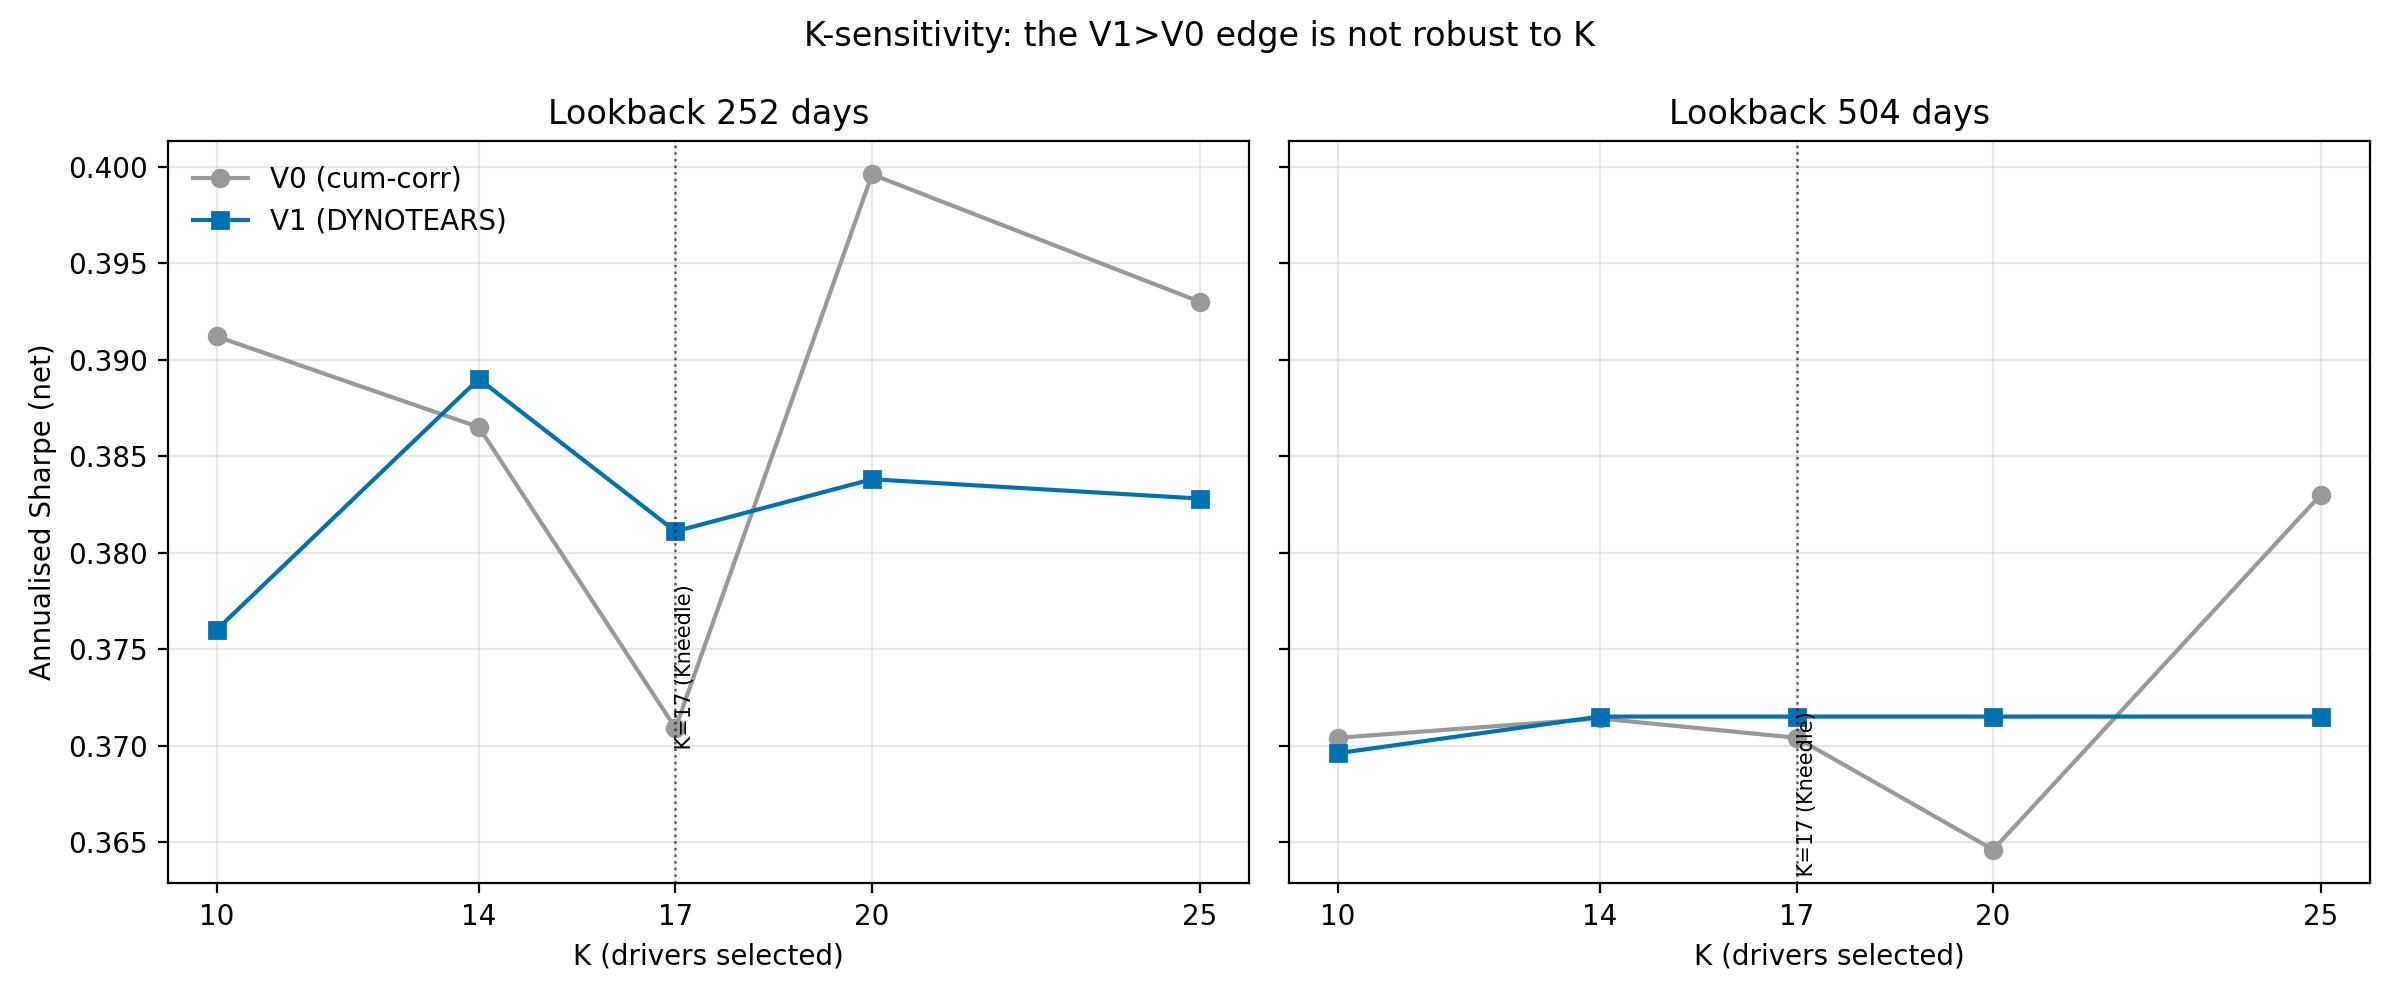
\includegraphics[width=0.97\textwidth]{figures/k_sensitivity.png}
  \caption{The driver route's $K$-fragility: net Sharpe of V0 and V1
    (DYNOTEARS) across the number of selected drivers $K$. The correlation
    selector's Sharpe varies erratically with $K$ while V1 is stable, so the
    sign of $V1-V0$ flips; V1 leads only near the calibrated $K=17$. No
    difference is significant.}
  \label{fig:ksens}
\end{figure}

\begin{figure}[tbp]
  \centering
  
\includegraphics[width=0.7\textwidth]{figures/feedback_grid.png}
  \caption{The closed loop is inert: V2 net Sharpe across the
    $\alpha\times\gamma$ feedback grid (one-year window) is $0.381$
    everywhere --- identical to open-loop V1 to four decimals. The feedback
    can only re-rank within the causally-selected set, and its monthly reward
    has signal-to-noise ${\approx}\,\rsRewardSNR$.}
  \label{fig:grid}
\end{figure}

\section{The decomposition: skeleton versus orientation}
\label{sec:decomposition}

\subsection{The headline split}

Figure~\ref{fig:decomp} is the dissertation's central result;
Table~\ref{tab:decomp} gives the numbers and Figure~\ref{fig:heatmap} the
full allocator--method matrix. At the \textbf{one-year window} the gain is
\emph{skeleton-dominated}: the skeleton contributes $+0.022$ ($p=0.14$) and
the best orientation increment adds only $+0.009$ on top (D1, $p=0.47$; D2s
$+0.003$, $p=0.80$; the remaining treatments are at or below D0). At the
\textbf{two-year window} the split \emph{inverts}: the skeleton's
contribution collapses to $+0.009$ ($p=0.55$) while orientation contributes
$+0.023$ (D1, pairwise $p=0.049$) to $+0.027$ (D2s, $p=0.067$) --- and all
five DYNOTEARS orientation-aware contrasts are positive
(Figure~\ref{fig:forest}). Family-wise, however, the orientation effect does
not survive: Hansen's SPA over the ten direction-aware variants against their
own skeleton control gives $p=\rsSpaDirWfive$ at two years (and
$p=\rsSpaDirWtwo$ at one year, where there is no effect to find).

\begin{figure}[tbp]
  \centering
  
\includegraphics[width=0.99\textwidth]{figures/phase_ii_decomposition.png}
  \caption{The answer to Q (DYNOTEARS graphs, net annualised Sharpe). At one
    year the causal graph's gain over the correlation control is carried by
    the skeleton; at two years the skeleton's gain collapses and orientation
    carries it. Steps annotated with the pairwise bootstrap $\Delta$ and
    $p$-value; no step survives family-wise correction.}
  \label{fig:decomp}
\end{figure}

\begin{table}[t]
  \centering
  \caption{The decomposition (DYNOTEARS): pairwise $\Delta$Sharpe with
    Politis--Romano $p$-values. The total splits by the shared anchor:
    total $=$ skeleton $+$ orientation.}
  \label{tab:decomp}
  \begin{tabular}{l c c}
    \toprule
    Contrast & Window 252 & Window 504 \\
    \midrule
    skeleton\quad (D0 $-$ \textsc{corr}) & $+0.022$ ($p=0.14$) & $+0.009$ ($p=0.55$) \\
    orientation, D1\quad (D1 $-$ D0)     & $+0.009$ ($p=0.47$) & $+0.023$ ($p=0.049$) \\
    orientation, D2s\quad (D2s $-$ D0)   & $+0.003$ ($p=0.80$) & $+0.027$ ($p=0.067$) \\
    \midrule
    total, D1\quad (D1 $-$ \textsc{corr})   & $+0.031$ ($p=0.14$) & $+0.032$ ($p=0.12$) \\
    total, D2s\quad (D2s $-$ \textsc{corr}) & $+0.026$ ($p=0.24$) & $+0.036$ ($p=0.084$) \\
    \bottomrule
  \end{tabular}
\end{table}

\begin{figure}[tbp]
  \centering
  
\includegraphics[width=0.99\textwidth]{figures/phase_ii_heatmap.png}
  \caption{Net Sharpe by discovery method $\times$ allocator at both windows
    (boxed column: the skeleton control D0). The one-year row is
    skeleton-strong; the two-year DYNOTEARS row is orientation-strong; the
    VARLiNGAM rows show no orientation effect at all.}
  \label{fig:heatmap}
\end{figure}

\begin{figure}[tbp]
  \centering
  
\includegraphics[width=0.99\textwidth]{figures/phase_ii_forest.png}
  \caption{The fixed-graph orientation effect: $\Delta$Sharpe of each
    orientation-aware allocator against the skeleton control D0, with
    $95\%$ block-bootstrap CIs ($\ast$: $p<0.05$). All five DYNOTEARS
    contrasts are positive at the two-year window; none is at one year, and
    none is under VARLiNGAM.}
  \label{fig:forest}
\end{figure}

\subsection{What is orientation actually buying?}

Not level, but \emph{consistency across estimation windows}. The skeleton
allocator's performance is window-fragile ($0.403 \to 0.372$); D1
($0.411/0.395$) and D2s ($0.406/0.399$) are the only allocators in the study
strong at both windows (Figure~\ref{fig:nav} shows the one-year NAV paths). A
mechanism consistent with this: at 504 days the sample covariance is
estimated over regimes it averages away, while
$\Sigma_{\mathrm{struct}}$ --- built from the contemporaneous graph and its
shock variances --- imposes the causal structure of the \emph{current} fit
window on the allocation, retaining information the long-window sample
moments blur. On this reading, orientation acts as a regulariser of the
allocation step rather than a source of extra return, which is exactly what
the level-vs-robustness pattern shows.

\begin{figure}[tbp]
  \centering
  
\includegraphics[width=0.99\textwidth]{figures/phase_ii_nav.png}
  \caption{Cumulative net NAV, one-year window: the correlation control, the
    HSP baseline V0, the skeleton D0, the orientation-aware D1 and D2s, and
    the driver route V1. All variants absorb the full ${\approx}51\%$ GFC
    drawdown --- the study concerns relative allocation quality, not
    drawdown avoidance.}
  \label{fig:nav}
\end{figure}

\subsection{Is the split robust to the design knobs?}

\paragraph{Sparsity ($\tau$).} Thresholding the graph at
$\tau\in\{0,0.01,0.05,0.10\}$ leaves the treatments flat-to-better (D2:
$0.399\to0.402$; D3: $0.397\to0.407$ at the heaviest threshold) while the
skeleton control drifts down ($0.403\to0.394$) --- the orientation-aware
allocators are not artefacts of the regularisation knob.

\paragraph{Costs and turnover.} The orientation increment is
cost-invariant: D1$-$D0 at two years moves from $+0.022$ to $+0.025$ as
costs rise from 0 to 20\,bps, because D1's turnover ($0.102$ one-way per
rebalance) is \emph{below} the control's ($0.112$); D3's is lower still
($0.066$). Orientation does not win by trading less, and is not eroded by
trading more.

\paragraph{Discovery method.} Under VARLiNGAM graphs the orientation effect
is absent everywhere (all contrasts ${\approx}0$ or negative;
Figure~\ref{fig:forest}, right). The decomposition is therefore
\emph{method-dependent}: DYNOTEARS' jointly-optimised, acyclicity-constrained
$W$ supports orientation-aware allocation where VARLiNGAM's ICA-ordered
$B_0$ does not --- consistent with VARLiNGAM's identification weakening as
residuals Gaussianise over longer windows. Under the deliberately cheap
GRANGER graphs the split is informative: causal-ordered bisection survives
(D2 $=0.393$ vs DYNOTEARS' $0.399$) but the structural-covariance allocators
collapse (D1 $=0.352$, D3 $=0.350$) --- a ridge-VAR coefficient matrix
supports an \emph{ordering} but its magnitudes cannot support shock
propagation. Expensive discovery earns its cost only for the allocators that
consume edge weights, and the best-allocator gap (GRANGER $-$ DYNOTEARS at
D1: $-0.060$, $p=0.12$) favours DYNOTEARS without reaching significance.

\subsection{Where does orientation help --- stress or calm?}
\label{sec:regimes}

The prior-verification result (Section~\ref{sec:discovery-run}) showed edge
\emph{assignment} matters most in stress windows, motivating the hypothesis
that orientation-aware allocation would earn its keep in crises. The
regime-conditional analysis rejects this (Figure~\ref{fig:regime}): at the
one-year window the orientation-aware allocators' edge over V0 concentrates
in the \emph{bottom} VIX quintile ($+0.22$/$+0.25$ Sharpe for D1/D2s) and is
approximately zero (D1) to negative (D2s) in the top quintile; in NBER
recessions the skeleton allocator is the strongest and D1 adds nothing. A
plausible reading is that in stress, correlations rise toward one and any
structure --- causal or correlational --- is swamped by the common factor,
while in calm markets cross-sectional causal heterogeneity is the signal;
but whatever the mechanism, the hypothesis as stated was wrong, and is
reported as such.

\begin{figure}[tbp]
  \centering
  
\includegraphics[width=0.9\textwidth]{figures/phase_ii_regime.png}
  \caption{Regime-conditional Sharpe excess over V0 (one-year window). The
    orientation-aware edge concentrates in the VIX bottom quintile (calm
    markets), not in stress: the stress hypothesis is rejected.}
  \label{fig:regime}
\end{figure}

\section{What survives rigour?}
\label{sec:believe-rigour}

% Numbers in this section come from _generated/robust_stats.tex, regenerated
% by `python -m scripts.robust_stats --phase-ii` over all evaluated bundles.

\paragraph{Non-normality and selection bias (PSR/DSR).} Every headline
allocator's Probabilistic Sharpe ratio (the probability its true Sharpe
exceeds zero given the sample's higher moments) is high --- \textsc{corr}
$\rsCorrPSR$, D0 $\rsVprimePSR$, D1 $\rsDonePSR$ at one year --- so the
\emph{levels} are not fat-tail artefacts. Deflating against the best Sharpe
expected from \rsNtrials\ no-skill trials, D1 attains the \emph{highest
Deflated Sharpe ratio in the entire study} ($\rsDoneDSR$, vs the control's
$\rsCorrDSR$ and the skeleton's $\rsVprimeDSR$), with D2s second among
allocators ($\rsDtwosDSR$). The ordering of the decomposition survives
deflation; its statistical separation does not, as the family-wise tests
show.

\paragraph{Family-wise comparisons (RC/SPA).} Four pre-specified SPA tests
adjudicate the report's claims with the search priced in. \textbf{(i)}
Causal-structure strategies vs the HSP baseline V0 at one year:
$p=\rsSpaConsistent$ --- significant, but as Section~\ref{sec:r1} showed,
substantially a verdict on V0's machinery. \textbf{(ii)} The same family vs
the \textsc{corr} control: $p=\rsSpaSkelWtwo$ (one year) and
$\rsSpaSkelWfive$ (two years) --- R1 not established family-wise.
\textbf{(iii)} Orientation-aware variants vs their own skeleton control:
$p=\rsSpaDirWtwo$/$\rsSpaDirWfive$ --- the orientation effect, suggestive
pairwise at two years, does not survive its own multiplicity.
\textbf{(iv)} The Phase-II variants against V0: $p=\rsSpaDvar$. The pattern
is coherent: every family-wise test that anchors on a \emph{weak} benchmark
(V0) rejects; every test that anchors on an honest one does not.

\paragraph{The Model Confidence Set.} The $90\%$ MCS over the
\rsMcsUniverse\ distinct one-year strategies retains \rsMcsSize\ of them,
eliminating only \rsMcsExcluded. Read correctly, this is a statement about
power, not a vindication of everything retained: with twenty-plus highly
correlated long-only variants whose Sharpes span $0.35$--$0.41$, the
equivalence test can only discriminate against the strategy that loses
\emph{consistently} --- the HSP baseline V0. The MCS confirms V0's
inferiority and otherwise declines to rank the causal family --- including
declining to separate treatments from controls.

\paragraph{The seed audit.}
\label{sec:seed-audit}
Re-running the committed driver-route configuration (V1, one-year window,
$K{=}17$) under \rsSeedN\ neural-network seeds --- discovery cached, so the
initialisation is the \emph{only} varying ingredient --- moves its net
Sharpe across $[\rsSeedMin, \rsSeedMax]$ (median $\rsSeedMedian$;
Figure~\ref{fig:seed}). The range ($\rsSeedRange$) is more than twice the
$+0.010$ edge the arm claims over its own baseline, and the committed value
sits at the $\rsSeedPct$th percentile of its own seed distribution --- at
the unluckiest seed the edge all but vanishes. This quantifies, on this
pipeline, the concern that neural sensitivity-based results are fragile to
undisclosed seed choices; and it is the strongest argument for the
deterministic D-family, every member of which sits \emph{above the seed
cloud's maximum} and produces byte-identical results on every run.

\begin{figure}[tbp]
  \centering
  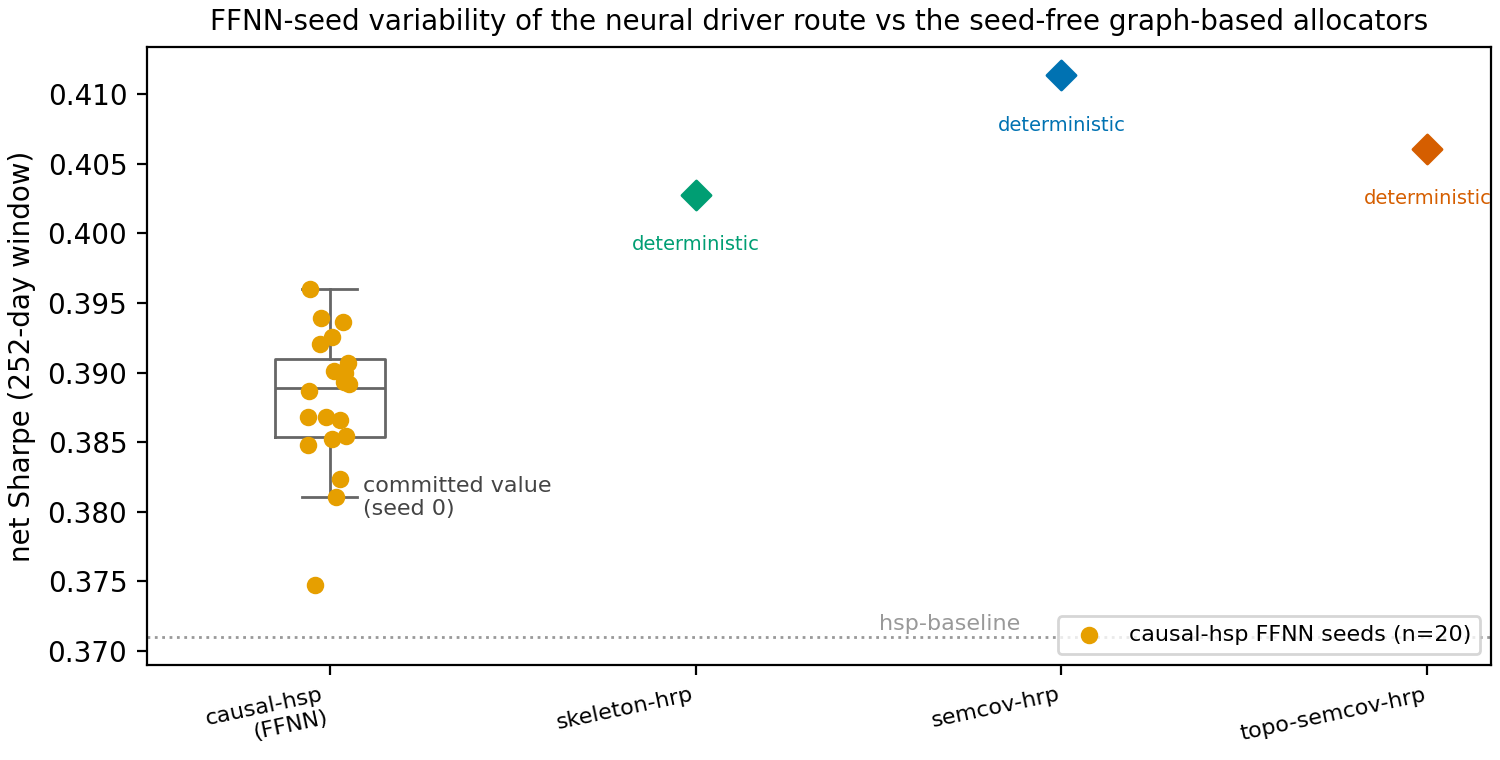
\includegraphics[width=0.85\textwidth]{figures/phase_ii_seed.png}
  \caption{The seed audit: net Sharpe of the driver route V1 across
    \rsSeedN\ network seeds (one-year window), against the deterministic
    graph-based allocators. The seed range exceeds V1's claimed edge over
    its baseline; every D-variant sits above the seed-cloud maximum.}
  \label{fig:seed}
\end{figure}

\paragraph{Verdict on Q, with uncertainty stated.} The decomposition's
\emph{point estimates} are clear and internally consistent: skeleton-carried
gain at one year, orientation-carried gain at two, with orientation acting
as a cross-window stabiliser and D1 topping the study-wide DSR table. Its
\emph{statistical support} is honest but thin: consistent signs across
twelve contrasts and two windows, one pairwise-significant cell
($p=0.049$), and no family-wise survival anywhere. The largest defensible
claim is conditional: \emph{if} one replaces the correlation matrix with a
DYNOTEARS graph, the skeleton is what pays at short windows, and keeping the
orientations costs nothing while materially improving robustness to the
estimation-window choice.

\section{How much should we believe this?}
\label{sec:believe}

\paragraph{Effect sizes sit near the detection floor.} The decomposition's
components are $0.01$--$0.03$ Sharpe over 18 years; at this sample length
such effects are at the edge of detectability, so the absence of family-wise
significance is not evidence of absence --- but equally the presence of one
$p=0.049$ cell among ten orientation contrasts is exactly what multiplicity
predicts under the null, which is why it is not claimed as a discovery.

\paragraph{Pre-registration limits, and residual garden-of-forking-paths
risk.} The allocator grid, contrasts and controls were fixed in a written
plan before any treatment cell ran, and no allocator was added afterwards;
but the plan itself was written after the first phase's results were known,
so the choice of \emph{question} was data-informed even though the
\emph{experiment} was not. The unified deflation universe (all \rsNtrials\
configurations ever evaluated, both phases) is the corrective applied.

\paragraph{Single asset class, one universe, approximated index.} Everything
here concerns long-only allocation within ${\sim}100$ US large-caps; every
variant absorbs the full ${\approx}51\%$ GFC drawdown. Whether the
decomposition transfers to universes with richer exogenous structure
(multi-asset, credit, commodities) is untested. The top-by-market-cap
approximation of the S\&P~100 and the fixed snapshot-union universe carry
mild residual survivorship effects.

\paragraph{Method-dependence is a caveat on the mechanism.} The orientation
effect exists under DYNOTEARS graphs only. Until a second discovery method
reproduces it, the safest interpretation is ``DYNOTEARS' contemporaneous
structure supports orientation-aware allocation'', not ``causal orientation
in markets is allocatively valuable''.

\paragraph{What the evidence supports, and does not.} It supports: the
graph's consistent, modest, direction-uniform improvement over the
correlation matrix; the window-dependent skeleton/orientation split; the
robustness role of orientation; and the dominance of deterministic
graph-based allocation over the seed-unstable, feedback-inert driver route.
It does not support: any family-wise-significant improvement over an honest
correlation control; any orientation effect under VARLiNGAM; or the stress
hypothesis. That asymmetry --- precise point estimates, honestly thin
inference --- is the finding.
